\section{Introduction}
\label{sec:introduction}
\lhead{\thesection \space Introduction}

This document is my individual reflection in the context of the module Software Factory, which is part of the Software Engineering course at Fontys University of Applied Sciences Venlo. The project that is reflected on concerns the application \textit{Connected.Football} as well the extension \textit{Vote4Fun}, which was developed over the course of this project.
\newline
As part of this module, students taking part in the course have to prove that their own competences regarding activities taking place in a software development project have improved by taking part in the project. The competences that had to be improved were defined at the beginning of the project and related to the role each student took while working on it. My role during the project was the role of \textit{Software Architect}.
\newline
As mentioned above, the competences were defined at the beginning of the module. This definition is part of my personal development plan, which can be found in \textit{Appendix \ref{appendix:personal_development_plan}: \nameref{appendix:personal_development_plan}}. Sections from this plan are references frequently in this document, to prove that the planned acquiry of competences did take place. Furthermore, this document follows almost exactly the same structure as the mentioned plan, for easier comparison.
\newline
To define competences, this reflection makes use of the model used to describe the Bachelor of ICT, which includes a competence matrix known as \textit{Body of Knowledge and Skills} (BOKS), as seen in Figure \ref{fig:boks}. This matrix includes both the activities as well as the architectural layers common in an ICT environment as its dimensions. Each combination of activity and architectural layer makes up a form of competence, which can be ranked in level of skill, on a scale of 1 to 3.

\begin{figure}[H]
    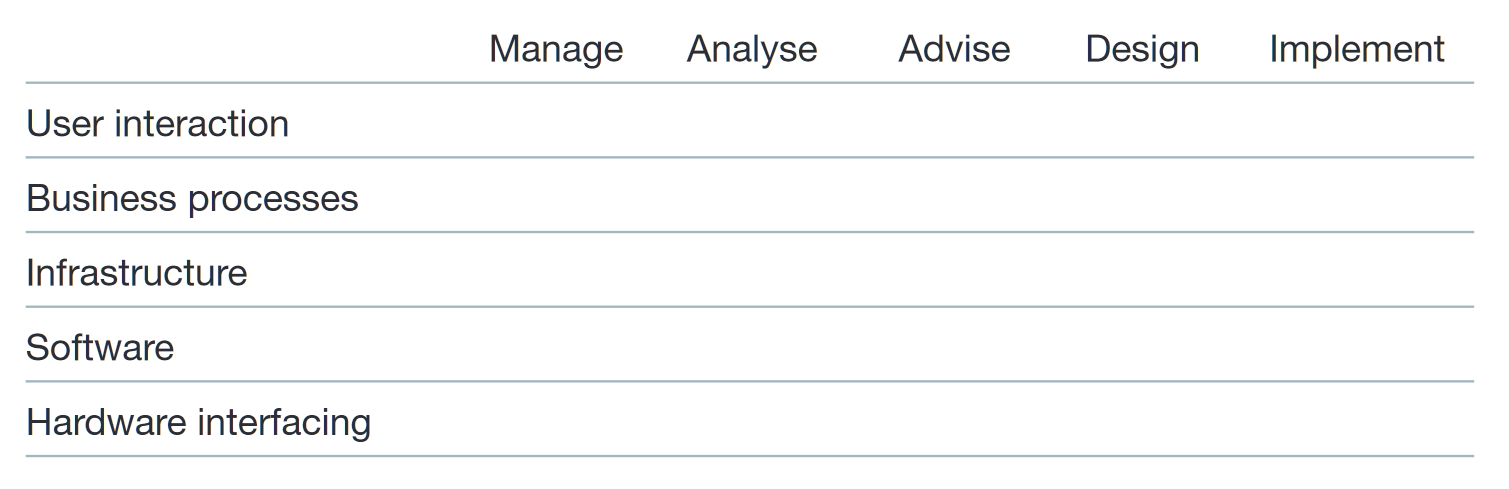
\includegraphics[width=\textwidth]{images/boks.png}
    \caption{Body of Knowledge and Skills}
    \label{fig:boks}
\end{figure}

This reflection covers three activities in a certain architectural layer listed in the Figure above. To do so, it is described what level of competence I possessed in executing each activity in one certain architectural layer at the beginning of the project and at the end of it. It is described what level the competence represents and why this current level of competence is justified. For each activity and architectural layer it is described what is necessary to qualify for such a level of competence and how the author learned these skills in the context of the project.